%%%%%%%%%%%%%%%%%%%%%%%%%%%%%%%%%%%%%%%%%%%%%%%%%%%%%%%%%%%%%%%
%
% Welcome to Overleaf --- just edit your LaTeX on the left,
% and we'll compile it for you on the right. If you give
% someone the link to this page, they can edit at the same
% time. See the help menu above for more info. Enjoy!
%
%%%%%%%%%%%%%%%%%%%%%%%%%%%%%%%%%%%%%%%%%%%%%%%%%%%%%%%%%%%%%%%
\documentclass{beamer}

\usetheme{Warsaw}
\usepackage{amsmath}
\usepackage{graphicx}

\title{Gettysburg Cemetery Dedication}
\author{Abraham Lincoln}
\institute{United States of America}
\date{19 Nov 1863}

\begin{document}

\begin{frame}
\titlepage
\end{frame}

\begin{frame}
\frametitle{Outline}
\tableofcontents
\end{frame}

\section{Agenda}

\begin{frame}
\frametitle{Agenda}
\begin{itemize}
\item Met on battlefield (great)
\item Dedicate portion of field --- fitting!
\item Unfinished work (great tasks)
\end{itemize}
\end{frame}

\begin{frame}
\frametitle{Not on Agenda!}
  \begin{itemize}
  \item Dedicate
  \end{itemize}
\end{frame}

\begin{frame}
\frametitle{Not on Agenda!}
  \begin{itemize}
  \item Dedicate
  \item Consecrate
  \end{itemize}
\end{frame}

\begin{frame}
\frametitle{Not on Agenda!}
  \begin{itemize}
  \item Dedicate
  \item Consecrate
  \item Hallow (in narrow sense)
  \end{itemize}
\end{frame}

\begin{frame}
\frametitle{Not on Agenda!}
  \begin{itemize}
  \item Dedicate
  \item Consecrate
  \item Hallow (in narrow sense)
  \item Add or detract
  \end{itemize}
\end{frame}

\begin{frame}
\frametitle{Not on Agenda!}
  \begin{itemize}
  \item Dedicate
  \item Consecrate
  \item Hallow (in narrow sense)
  \item Add or detract
  \item Note or remember what we say
  \end{itemize}
\end{frame}

\section{Review}

\begin{frame}

\frametitle{Key Objectives \& Success Factors}

\begin{itemize}

\item What makes nation unique

\begin{itemize}

\item Conceived in Liberty
\item Men are equal

\end{itemize}
  
\end{itemize}

\begin{block}{Shared vision}

\begin{itemize}

  \item New birth of freedom.
  \item Gov't of/for/by the people.

\end{itemize}

\end{block}
  
\end{frame}

\begin{frame}

\frametitle{Organizational Overview}

\begin{figure}
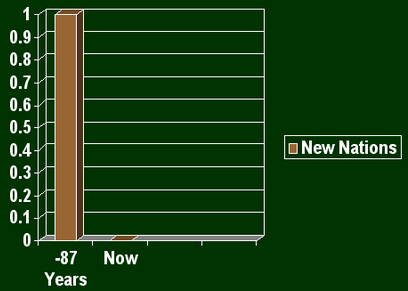
\includegraphics[width=0.5\textwidth]{gettysburg_graph.png}
\end{figure}

\begin{block}{Four Score and Seven}

\begin{equation}
-(4 \times 20 + 7) = -87
\end{equation}

\end{block}

\end{frame}

\section{Summary}

\begin{frame}

\frametitle{Summary}

\begin{columns}

\begin{column}{0.4\textwidth}

\begin{itemize}
\item New nation
\item Civil war
\item Dedicate field
\end{itemize}

\end{column}

\begin{column}{0.6\textwidth}

\begin{itemize}
\item Dedicated to unfinished work
\item New birth of freedom
\item Government not perish
\end{itemize}

\end{column}

\end{columns}

\end{frame}

\end{document}